\documentclass[border=10pt,varwidth]{standalone}
\usepackage{tikz}
\usetikzlibrary{shapes,arrows,shapes.multipart, positioning}

\begin{document}

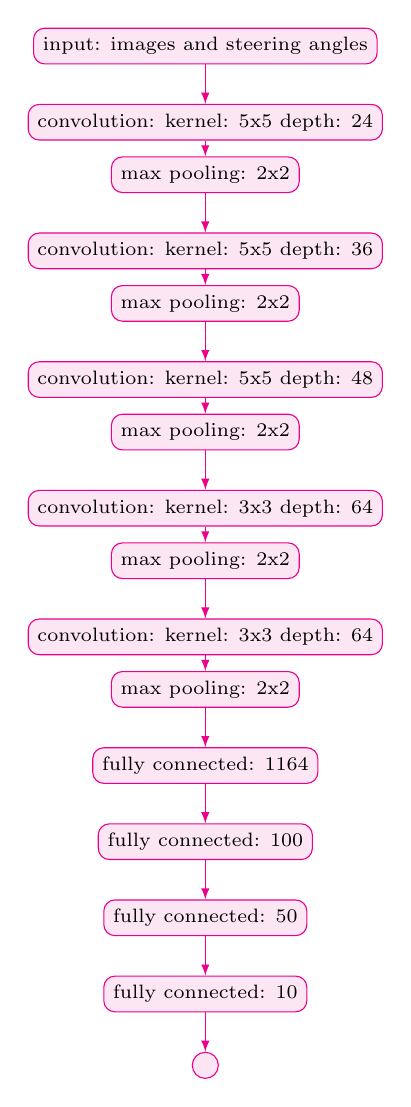
\begin{tikzpicture}
    \tikzset{
        node/.style = {rectangle, draw=magenta,  fill=magenta!10, thin, rounded corners},
        line/.style = {draw=magenta, thin, -latex},
        output/.style = {circle, draw=magenta,  fill=magenta!10, thin},
    }
    
    \node[node](input){\scriptsize input: images and steering angles};
    
    \node[node](conv1)[below = 0.5cm of input]{\scriptsize convolution: kernel: 5x5 depth: 24};
    \node[node](pool1)[below = 0.2cm of conv1]{\scriptsize max pooling: 2x2};
    
    \node[node](conv2)[below = 0.5cm of pool1]{\scriptsize convolution: kernel: 5x5 depth: 36};
    \node[node](pool2)[below = 0.2cm of conv2]{\scriptsize max pooling: 2x2};
    
    \node[node](conv3)[below = 0.5cm of pool2]{\scriptsize convolution: kernel: 5x5 depth: 48};
    \node[node](pool3)[below = 0.2cm of conv3]{\scriptsize max pooling: 2x2};
    
    \node[node](conv4)[below = 0.5cm of pool3]{\scriptsize convolution: kernel: 3x3 depth: 64};
    \node[node](pool4)[below = 0.2cm of conv4]{\scriptsize max pooling: 2x2};
    
    \node[node](conv5)[below = 0.5cm of pool4]{\scriptsize convolution: kernel: 3x3 depth: 64};
    \node[node](pool5)[below = 0.2cm of conv5]{\scriptsize max pooling: 2x2};
    
    \node[node](fc1)[below = 0.5cm of pool5]{\scriptsize fully connected: 1164};
    \node[node](fc2)[below = 0.5cm of fc1]{\scriptsize fully connected: 100};
    \node[node](fc3)[below = 0.5cm of fc2]{\scriptsize fully connected: 50};
    \node[node](fc4)[below = 0.5cm of fc3]{\scriptsize fully connected: 10};
    
    \node[output](output)[below = 0.5cm of fc4]{\scriptsize };    
    

    \path [line] (input) -- (conv1);
    \path [line] (conv1) -- (pool1);
    
    \path [line] (pool1) -- (conv2);
    \path [line] (conv2) -- (pool2);
    
    \path [line] (pool2) -- (conv3);
    \path [line] (conv3) -- (pool3);
    
    \path [line] (pool3) -- (conv4);
    \path [line] (conv4) -- (pool4);
    
    \path [line] (pool4) -- (conv5);
    \path [line] (conv5) -- (pool5);
    
    \path [line] (pool5) -- (fc1);
    \path [line] (fc1) -- (fc2);
    \path [line] (fc2) -- (fc3);
    \path [line] (fc3) -- (fc4);
    
    \path [line] (fc4) -- (output);

\end{tikzpicture}

\end{document}
